\subsection{Transfer grid velocities to particles}

As we could see in the previos section, going from particle velocities to grid can be a bit tricky when working with a MAC grid. Luckily, going from grid velocities to particle velocities is a lot easier. For every particle, we will use bilinaer interpolation to get the horizontal and vertical velocities.

\begin{figure}[ht!]
\centering
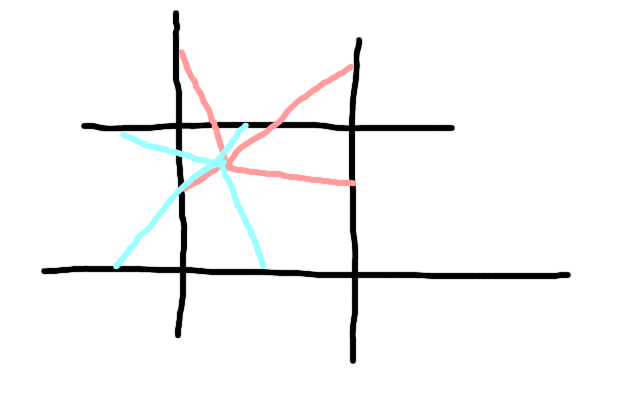
\includegraphics[width=80mm]{ch3/bilerp.png}
\caption{A simple caption}
\label{onedge}
\end{figure}

The FLIP approach to overall simulation implementation is how we update the particle velocities. If we only update the particles with the velocities that the pressure solver gives us, then it is not FLIP but PIC, Particle in Cell which is an older approach. Zhou and Bridson are in their report, before solving the pressure equations, saving the old divergence-free velocity field and then updating the particles with the change of velocity instead of only the new velocity.

\begin{equation}
\Delta \vec{u} = \vec{u}^{n+1} - \vec{u}^n
\end{equation}

FLIP alone can cause a lot of noise because of the many particles and it was recommended to linearly interpolate between FLIP and PIC for best result. To formula for new particle velocities are then

\begin{equation}
\vec{u}_p = \alpha \cdot bilerp(\vec{u}^{n+1}, \vec{x}_p) + (1-\alpha) \cdot bilerp(\Delta \vec{u},\vec{x}_p)
\label{flipeq}
\end{equation}

where $\alpha$ is a number between $0$ and $1$. If one, then it's pure PIC and if zero then it's entirly FLIP. Lower values gives a more stable look but to the cost of more numerical dissipation which cancels out a lot of the interesting high frequency motion.
